\chapter{Skin Data Analysis}
In this chapter first the anatomy of human skin, then the cutaneous melanoma and its different types as well as its clinical diagnosis are discussed. Later common imaging techniques for diagnosis of melanoma are discussed. Finally at the end skin optical properties and different methods for modeling light propagation through skin are reviewed. 



	


	
	
	\subsection{Clinical Diagnosis}
	%% ABCD, ABCDE, 7 check point list , Biopsy, Melanoma stages, staging factors
Due to visible nature of melanoma disease, visual inspection of the lesions is the first step of diagnosis. The visual inspection is based on certain criteria with the aim to differentiate between benign and suspicious lesions. In 1985 Friderman et al. \cite{Friedman1985} introduced ``ABCD'' criteria for identifying melanoma. This method introduced simple criteria for appraise of one lesion such as Asymmetry, Border irregularity, Color variegation and Diameter greater than 6 mm.  Due to its simple definition of the criteria, this method have been used widely in clinical practice. However later in 2004, Abbasi et al. \cite{Abbasi2004} proposed expanding the ``ABCD'' criteria to ``ABCDE'', while E stands for evolving the lesion over time with respect to size, shape, shades of color, surface features or symptoms. \\

 Clasgow 7-point checklist \cite{Mackie1991} is another melanoma identification method in clinical diagnosis. This method considers three major criteria such as changes in size, shape and colors and four minor criteria, including diameter greater than 7 mm, inflammation, crusting or bleeding and sensory change. Opposed to ABCDE and ABCD, Glosgow 7 point checklist is not widely adopted and the used of the former method is more evident in the state of the art. 
 
%%Beside what is mentioned here, it is often to see the same technical terms (ABCD and 7-point checklist) in the literature, while they stand for different image modalities \cite{korotkov2012computerized}. For instance in the ABCD rule of dermoscopy, B stands for Border sharpness and D for Differential structure.  

All the mentioned methods are used by the dermatologists and non dermatologists to identify suspicious lesions and differentiate the benign melanocytic tumors from melanoma. The suspicious lesions are removed by biopsy and special measurements are conducted for evaluating the risk factor of the lesion.


 Based on American Joint Commission on Cancer (AJCC) (7th edition on melanoma staging and classification) \cite{balch2009final}, 10 different stages of melanoma are recognized in clinical and pathological used. This information is shown in Table \ref{T:Melanoma Sataging}. According to \cite{balch2009final}, there are several factors for determining the stage of melanoma and its indication, such as: 
	\begin{itemize}
	\item T- Tumor thickness. This factor varies from 1 - 4 and depending on the presence or absence of ulceration have different notation (b-a, respectively).
	\item N- Nodes (Lymph). This factor has 4 forms (0-3) and indicates if the melanoma has spread to lymph nodes.
	\item Metastasized. This factor points out if the cancer spread to other organs.
	\item Mitotic Rate, This parameter corresponds to the ratio of cell numbers in mitosis to total amount of cells and it is expressed as the number of mitoses/mm2.  
	\end{itemize}


	\begin{table}
	\small
	\caption{Melanoma Stages\cite{balch2009final}}
	\begin{center}
		\begin{tabular}{|c|p{8cm}|}
		\hline
		 Stage & Description \\ \hline
		 & \\
		 0 &  The tumor is bound to the epidermis and has not entered the dermis\\
		 & \\
		 IA & The tumor is less than 1 mm thick without ulceration (\textit{T1a}) and it has not spread to any other lymph nodes or organs (\textit{N0}, \textit{M0})\\
		  & \\
	     IB & The tumor is either less than 1 mm with the presence of ulceration (\textit{T1b}) or 1-2 mm and without ulceration (\textit{T2a}) and it is not spread to any other lymph nodes or organs (\textit{N0}, \textit{M0})\\
		 & \\
         IIA & The tumor is either between 1-2 mm and ulcerated (\textit{T2b}) or 2-4 mm thick and not ulcerated (\textit{T3a}. The tumor is not extended to other lymph nodes or organs (\textit{N0}, \textit{M0})\\
		 & \\
		 IIB & The tumor thickness is either 2-4 mm while ulcerated (\textit{T3b}) or more than 4 mm and not ulcerated (\textit{T4a}). The tumor has not spread to any lymph nodes or organs (\textit{N0}, \textit{M0})\\
		 IIC & The tumor is more than 4 mm thick and ulcerated (\textit{T4b}). The tumor has not extended yet to other parts of the body (\textit{N0}, \textit{M0})\\
		 & \\
         \pbox{2cm}{IIIA\\IIIB\\IIIC} & In this stage the tumor can be any thickness with presence or absence of ulceration (\textit{T $>$ T0}). The tumor has not spread to any other organs (\textit{M0}), however it is extended to the surrounded lymph nodes (\textit{N $>$ N0}).\\
         IV &  The cancel cells are extended to the other nodes and body organs. \\
 
         \hline
				  
		\end{tabular}
    \end{center}
	\label{T:Melanoma Sataging}	
	\end{table}	 
  
The mentioned factors are used to classify and stage melanoma, however two common indicators are mostly used to evaluate the progression of melanoma \cite{balch2009final}, including: 

	\begin{itemize}
	\item Clark's level\\
	The clark's level indicate the depth that the tumor is penetrated into the skin. Although it was shown that this diagnosis was not a great indicator, it is still used along the Breslow thickness. 
		\begin{itemize}
		\item Clark's level I - Bound to the epidermis (\textit{in situ} melanoma)
		\item Clark's level II - Confined to the upper part of papillary dermis 
		\item Clark's level III - Filling to the lower part of papillary dermis
		\item Clark's level IV - Invading to the reticular dermis
		\item Clark's level V - Expanding to the subcutaneous tissue
		\end{itemize}	
	
	\item Breslow thickness\\
The Breslow thickness indicates the vertical depth of the tumor in millimetres. This continuous factor is more accurate compare to Clark's level and is measured using an instrument called ocular micrometer \cite{balch2009final}. 
The research has shown there is a common relation between the Breslow thickness and the survival rate. 
		\begin{itemize}
		\item Breslow thickness $<$ 1 mm, 5- year survival is 95-100 \%
		\item 1 mm $<$ Breslow thickness $<$ 2 mm, 5- year survival is 80-96 \% 
		\item 2.1 mm $<$ Breslow thickness $<$ 4 mm, 5- year survival is 60-75 \%
		\item Breslow thickness $>$ 4 mm, 5- year survival is  37-50 \%
		\end{itemize}
	\end{itemize}

	\section{Imaging Techniques}
	%for the diseases altering its appearance.
	Skin is the largest organ of the body and can be examined directly by specialists. Due to this nature, visual inspection is the first procedure performed by dermatologists. In order to achieve spatially, uniform information for diagnostic purposes, different non-invasive imaging systems have been used in this field. These techniques allow the visualization of different skin structures however depending on their portability and ease of access by dermatologists, some have been used in daily basis, while the others are mostly used for research purposes. 
	The imaging systems based on ultraviolet (UV), visible (VIS), and near-infrared (NIR) spectrum, such as digital imaging, dermoscopy, multispectral, spectrophotometer and hyperspectral systems belong to the former group, while other imaging techniques including, optical coherence tomography (OCT), magnetic resonance imaging (MRI), high frequency ultrasound imaging and position emission tomography (PET) belong to the later group of non-invasive imaging systems. 
	This research is restricted to the images obtained by multispectral imaging and dermoscopy.
	
	\subsection{Multispectral Systems}
	Multispectral (\textit{MS}) system can be used either to capture a spectral information (\textit{Spectrophotometry}) or combination of spatial and spectral information (\textit{MS Imaging}). 
	
	Spectrophotometry, or in-vivo optical spectroscopy is a technique that proves to be potentially useful for clinicians. The reflectance spectrum is measured via a spectrophotometer and provides precise physical information of the object which are beyond the capability of human vision \cite{jolivot2011developpement}. Spectrophotometry is based on interaction of molecules with electromagnetic radiations and it is influenced by the absorption, scattering and emission properties of the skin. The spectral measurements as a results of spectrophotometer are independent of illumination change or metamerism condistions, since they are directly linked to the physical property of the studied object. Different spectrophotometry systems can be used such as diffused reflectance spectroscopy, fluorescence, Raman and multimodal spectroscopy.\\
	
		\begin{figure}
		\centering
		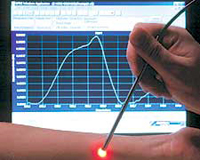
\includegraphics[width = 0.35\textwidth]{Chapter2/Figures/DRS.jpg}	
		\caption{Diffuse reflectance spectroscopy, Reflectance and absorption of light in skin}
		\label{fig:DRS}
		\end{figure}
	
	Multispectral imaging refers to a series of images captured at different wavebands across the electromagnetic spectrum. The wavebands can range from Ultra-Violet (UV) to InfraRed (IR). Using this advantage the multispectral image can contain more information beyond human eye capability. Such informations with respect to multilayer structure of the skin can be very useful. By using different wavelengths, the light is able to transfer in different depths and reveal various features related to skin layers.
Opposed to standard colour camera which is able to capture the skin image in three channel of (red, green, blue), multispectral imaging system acquires a sequence of gray level images at different wavelengths. This extended spectral capacity provides a high advantage in skin imaging since it is reducing the effects of metameric mismatches, which may occur due to different illumination and variability of sensor spectral responses \cite{jolivot2011developpement}.
	The spectral device of multispectral system, can be placed either in incident path, or in detection path. In either way, the main motivation is to go beyond the limited red, green and blue colour information which are available by other imaging techniques. This technique combines the advantage of both spectrophotometer and digital camera. The MS system acquire three dimensional data, the spatial information in 2 dimension and a spectral information in third dimension. Such system provides the spectral information for each pixel in the image. 	
	
	
	The MS imaging systems are further discussed in Chapter \ref{CH:MS}.


%A new category, called HyperSpectral Imaging (HSI) system is currently investigated
%by several research groups, mainly in microscopy [Ornberg et al., 1999] [Rothmann et al.,
%1998] and also for in-vivo optical diagnosis [Vo-Dinh et al., 2004]. However limitations
%of HSI are generally their complexity, cost and acquisition time [Balas et al., 2001] which
%may be affected by camera displacement. MSI and HSI systems are different because
%MSI systems generally involve 4 to 20 spectral bands when HSI systems are capable of
%recording higher number of very narrow spectral bands (20 - 100) [Vo-Dinh et al., 2004];
%hence the spectral resolution is higher for HSI.
%Figures 2.21(a),2.21(b),2.21(c),2.21(d) are the decomposition into spectral bands of a
%skin lesion. The figures provide the different spectral channels given respectively by the
%eyes, a RGB camera, a MSI system and a HSI one. It highlights that the amount of
%spectral information about skin lesions is gradually increased from digital colour camera
%to HSI.
%Most of MultiSpectral and HyperSpectral Imaging techniques require several exposures
%to acquire a data cube. Therefore, the acquired data have to justify the extra-time/cost
%in comparison to colour camera that acquires an image with a single exposure. When
%spectral acquisition is preformed successively, stacking together spectral data acquired
%even at short period of time might be affected by motion artefact. The justification is
%provided by the increased amount of information available about the skin reflectance not
%seen by the human eye.
%Once a spectral image is acquired, several mathematical approaches ranging from spa-
%tial to spectral can be used to analyse the data. The analysis can be performed on the
%spectral image (corrected after calibration) or this image can be transformed from a spec-
%tral image to a reflectance cube. The state of the art of skin analysis techniques are
%presented in chapter 4. In the following chapter, we present our own imaging system for
%dermatological applications.

	
	\subsection{Dermoscopy}
	Dermoscopy initially referrers to a non-invasive surface microscopy technique which is used for in vivo examination of epidermis and papillary dermis\cite{soyer1987early}. Dermoscopy brings new morphological criteria for differentiation of melanoma compared to other melanocytic and non-melanocytic pigmented skin lesions. A dermoscope can be seen similar to a magnifying lens which might contains extra features such as a built-in illumination system, a higher magnification and polarized filters. The principle of dermoscopy is transillumination which throws a strong light through an organ or part of skin as a mean of diagnosis of a skin area. This technique uses the fact that light incident on skin experiences reflection, refraction, diffraction and absorption and the physical properties of the skin are the source of these phenomena. Dermoscopy allows visualization of subsurface structures of dermis and papillary dermis which is not apparent to the unequipped eye by elimination the skin reflections from detected information. 
 Elimination of skin reflections can be achieved by applying linkage fluid to the skin, or using polarized light and polarized filters. \\
 Depending on the source light dermoscopy can be divided into two category, conventional Non-Polarized light contact dermoscopy (NPD), Polarized light dermoscopy (PD). The former category further can be divided into two group of polarized contact dermoscopy (PCD) or non-contact polarized dermoscopy(PNCD). Figure \ref{fig:NPD-PD} shows skin lesion images acquired with NPD and PD and Fig. \ref{fig:NPD-PD-NCPD} compares images of melanoma lesion via clinical imaging, non polarized dermoscopy, polarized light contact dermoscopy and polarized light non-contact dermoscopy \cite{Benvenuto-Andrade2007}

	\begin{figure}
	\centering
	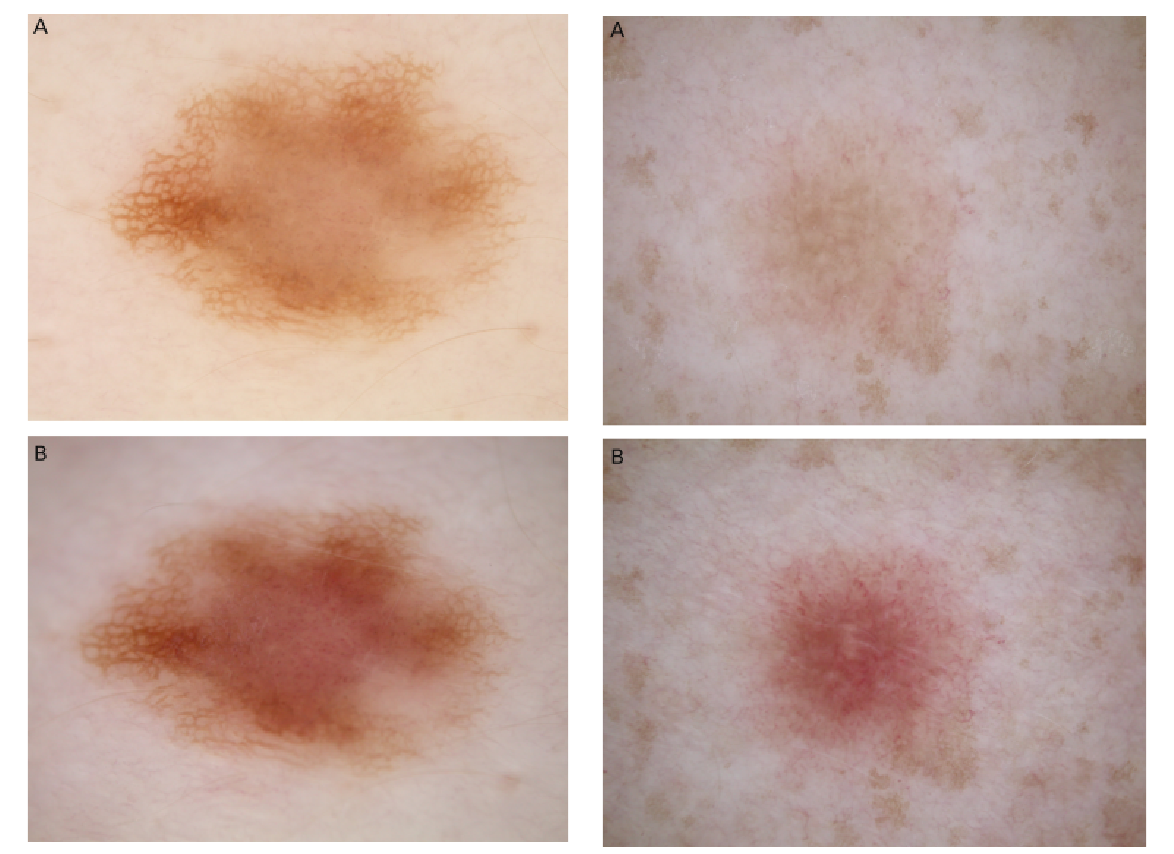
\includegraphics[width = 0.6\textwidth]{Chapter2/Figures/NPD_PD_01.png}	
	\caption{The images of atypical nevus (left) and MM lesion (right) with non polarized dermoscope(NPD, first row) and polarized dermoscope(PD, second row)\cite{wang2008differences}}
	\label{fig:NPD-PD}
	\end{figure}	 
	
	\begin{figure}
	\centering
	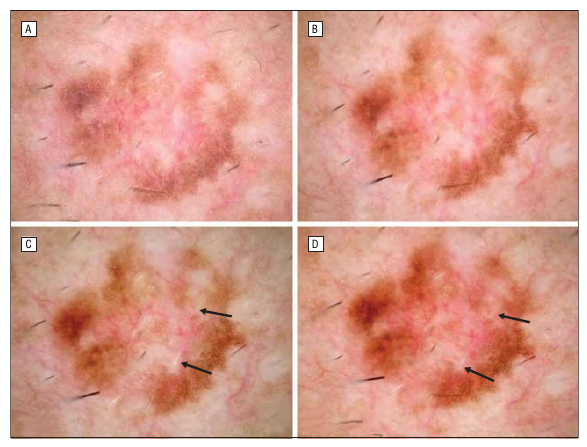
\includegraphics[width = 0.6\textwidth]{Chapter2/Figures/Clinic_NPD_PD_NCPD.png}	
	\caption{(A) A melanoma shown by clinical photography, (B) nonpolarized light contact dermoscopy (NPD),
(C) polarized light contact dermoscopy, (D) and polarized light noncontact dermoscopy. This melanoma had evidence of regression (fibrosis) on histopathological examination. Shiny-white streaklike areas within the melanoma (arrows in C and D), believed to represent fibrosis, are visiblein order to obtain full 2D image of any sample in short time.  under polarized but not NPD\cite{Benvenuto-Andrade2007}}
	\label{fig:NPD-PD-NCPD}
	\end{figure}	 
	
	
The NPD dermoscopy is also referred as \textit{in vivo cataneous surface microscopy}, \textit{magnified oil immersion  diascopy} and most commonly \textit{epiluminescence microscopy (ELM)}. This technique gets use of a hand held incident light, magnifying device (microscope) and immersion liquid in order to provide translucent surface of the skin and eliminates the reflections. The goal is to eliminate the surface scattering by minimizing the change of refractive index at skin/air interface. Immersion liquids such as oil, water or alcohol, has a refraction index relatively similar to skin and have been applied on skin surface prior to imaging. The contact between the skin and the glass interface of microscope is necessary in this case. The refractive of the glass is also very similar to the skin. 
The whole system, makes the stratum corneum of the skin translucent and reduces the amount of reflection at the skin surface. 

	\begin{figure}[h]
	\centering
	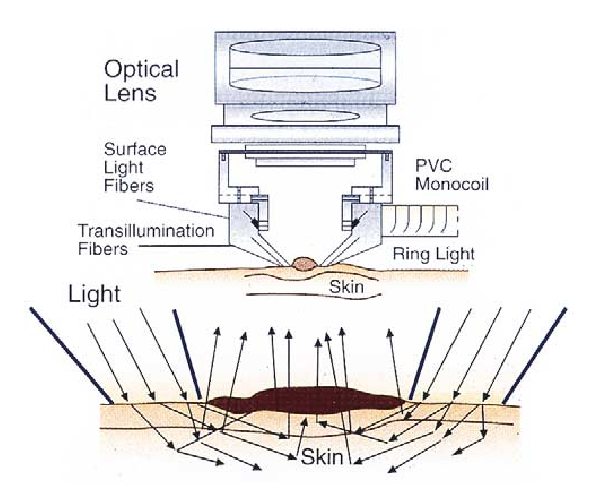
\includegraphics[width = 0.5\textwidth]{Chapter2/Figures/Nevoscope.png}	
	\caption{Dermoscopy functions by transillumination oflesion (Nevoscope)\cite{Marghoob2003}}
	\label{fig:Nevoscope}
	\end{figure}

The PD dermoscope consists of polarized light and two cross polarized filters in order to block the reflected lights and passing the scattered lights with in skin through the lens. One horizontal linear polarized filter is mounted in front of the source light, while the other filter, vertical linear polarized filter, is mounted in front of the detector. This allows for almost complete elimination of the reflection. 
Although the direct contact for the NPD and PCD is necessary, for PNCD there is no need for liquid interface neither direct contact.


Another imaging techniques, related to dermoscopy is the transilumination technology (TLM). This technique is patented and used only for a device called \textit{Nevoscope} (see Fig.\ref{fig:Nevoscope}) In this technique, the light is directed to the skin in such a way that allows the backscattered light illuminates the lesion from with in \cite{Patwardhan2003,patwardhan2004multi,patwardhan2005monte}.\\



	\section{Skin Optical Properties}
	 
Skin has two main optical properties which are absorption and scattering. If we assume an incident light with close incidence angel to normal, only \% 5 of the incident light is directly reflected at the surface, while the rest of the light is entered in the skin and goes through absorption and scattering phenomena. This pathway is also shown in Fig. \ref{fig:pathwayofLight}
	\begin{figure}[h]
	\centering
	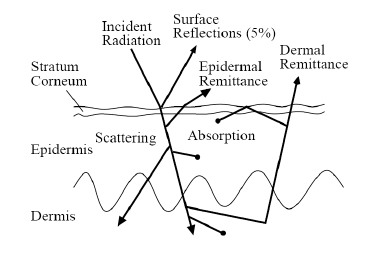
\includegraphics[width = 0.45\textwidth]{Chapter2/Figures/PWofLightinSkin.png}	
	\caption{Pathway of incident light in skin \cite{storring2000estimation}}
	\label{fig:pathwayofLight}
	\end{figure}

	Melanin and haemoglobin are the two important chromophores which play important part in appearance of normal skin and are responsible for absorbing the light. These chromophores strongly absorb light in the ultraviolet (UV) and visible ranges and have low absorption rate near-infrared range.	 
%Melanin is the major chromophore of the epidermis which occupies the top 50-100 \micro\meter, with the exception to superior layers of epidermis. Melanin is produced by melanosomes when exposed with UV light and is divided into two  types eumelanin and pheomelanin. Eumelanin has black/brown colour while pheomelanin has red/yellow colour. Concentration of this components are different between individuals, leading to different colour skins. 

%Haemoglobin is a chromophore of red colour found in the microvascular network of the dermis, typically 100-500 \micro\meter below the skin surface. This chromophore caries oxygen through vessels and capillaries. This chromophore accordingly is called oxy-haemoglobin while it contains oxygen and deoxy-haemoglobin otherwise.
	The absorption phenomenon correspond to the energy attenuation of a photon due to the absorption of a particle or a group of particles. The absorption coefficient of a layer is a function of the molar concentration and the absorption coefficient of the molecules presented in that layer. Meglinski et al \cite{meglinski2002quantitative} had defined the absorption coefficients of the single layer by set of equations as follows:
	\begin{equation}
	\footnotesize	
	\mu_{a}(\lambda)= \sum_{i=1}^{m}\big(\mu_{a}^{(i)}(\lambda)C_{i}\prod_{j=1}^{i-1}(1-C_{j})\big)+\mu^{(0)}(\lambda)\prod_{j=1}^{i-1}(1-C_{j})
	\label{Eq:AbsorptionCoefficient}
	\end{equation}

	\begin{equation}
	\footnotesize
	\begin{split}
	\mu_{a}^{layer}(\lambda)= (1-S) \gamma C_{blood} \mu_{a}^{Hb}(\lambda) + 
	S\gamma C_{blood}\mu_{a}^{HbO_{2}}(\lambda) + \\
	(1-\gamma C_{blood})C_{H_{2}O} \mu_{a}^{H_{2}O}(\lambda) + (1-\gamma C_{blood})(1-C_{H_{2}O})\mu_{a}^{(0)}(\lambda) 
	 \end{split}
     \label{Eq:AbsorptionCoefficientLayer}
	 \end{equation}
	 \begin{subequations}
	\begin{center}
	\begin{align}
	\mu_{a}^{(0)}(\lambda)= 7.84 \times 10^{7} \times \lambda ^{-3.255}\\
	\gamma = F_{Hb} F_{RBC} H_{t}	
	\end{align}
	\end{center}
	\label{Eq:AbsorptionCoefficientmuandgamma}
	\end{subequations}	 

	In the above equations, $C_{i}$ is the volume fraction of the $i^{th}$ molecule, $m$ is the total number of molecules in the layer, $\mu_{a}^{(i)}$ is the absorption coefficient of the $i^{th}$ absorber and $\mu^{(0)}$ is the absorption coefficient of the medium without absorber. $\mu_{a}^{H_{2}O}$, $\mu_{a}^{HbO_{2}}$ and $\mu_{a}^{Hb}$ are the absorption coefficients of water, oxy and deoxy haemoglobin respectively and their values over the VIS and NIR spectrum (400–1100 nm) 
are shown in Fig.\ref{fig:waterabsorptioninSkin}. $C_{blood}$ and $C_{H_{2}O}$ are the layer volume fractions of blood and water (see Table \ref{T:MeglinskiTable}).  $S$ is the oxygen saturation in blood and is assumed to be constant at 0.6. $\gamma$ is the total fractions of haemoglobin in blood and can be calculated using three parameters of $F_{Hb}$ (volume fraction of haemoglobin in an erythrocyte),  $F_{RBC}$ (volume fraction of erythrocytes in the total volume
of all blood cells) and $H_{t}$ (the haematocrit). The values of these parameters were considered constant such as: 0.25, 0.99 and 0.45 respectively. \\
	
	\begin{table}
	\caption{The parameters used in the skin model defined by \cite{meglinski2002quantitative}}
	\begin{center}
	\footnotesize
	\begin{tabular}{ c c c c c c c}
	\hline 
	k &  $\#$ Layers & $C_{blood}$ & $C_{H_{2}O}$ & $\mu_{s}$($mm^{-1}$) & g & n \\
	\hline 
	1 & Stratum corneum & 0 & 0.05 & 100 & 0.86 & 1.5 \\
	2 & Living epidermis & 0 & 0.2 & 45 & 0.8 & 1.34 \\
	3 & Papillary dermis & 0.04 & 0.5 & 30 & 0.9 & 1.4 \\ 
	4 & Upper blood net dermis & 0.3 & 0.6 & 35 & 0.95 & 1.39 \\ 
	5 & Reticular dermis & 0.04 & 0.7 & 25 & 0.8 & 1.4 \\
	6 & Deep Blood net dermis & 0.1 & 0.7 & 30 & 0.95 & 1.38 \\
	7 & Subcutaneous fat & 0.05 & 0.7 & 5 & 0.75 & 1.4 \\
	\hline 	  
	\end{tabular}
    \end{center}
	\label{T:MeglinskiTable}	
	\end{table}
	
	\begin{figure}
	\centering 
	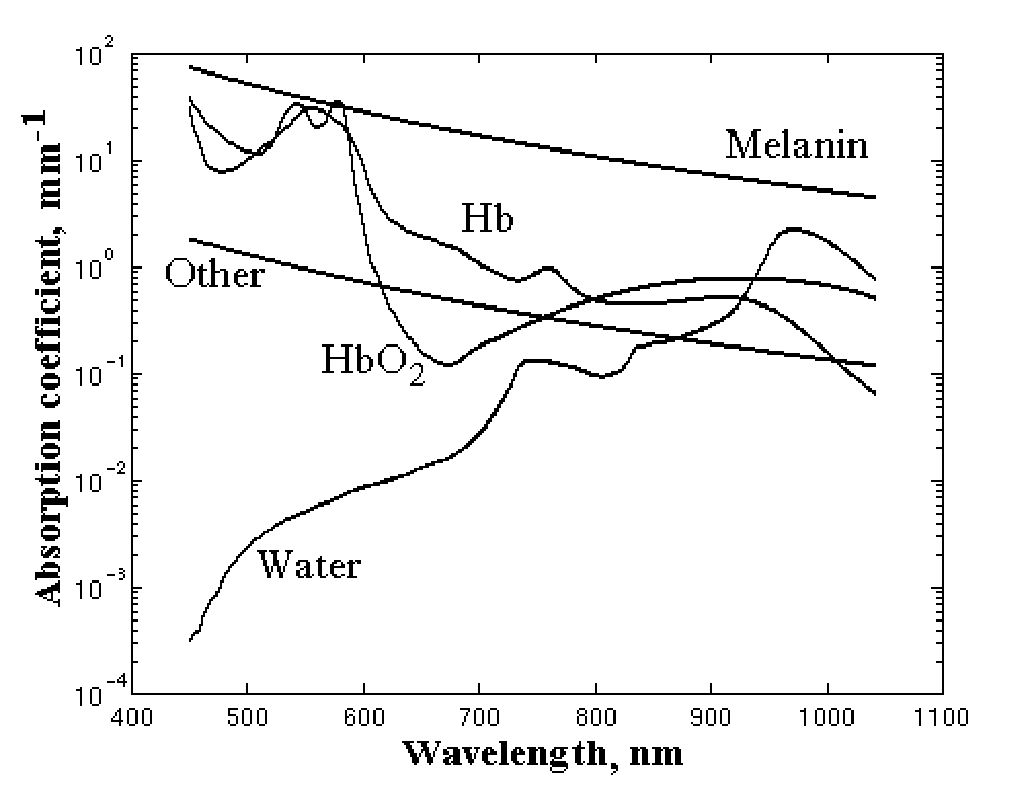
\includegraphics[width = 0.6\textwidth]{Chapter2/Figures/AbsorptionCoeff.png}	
	\caption{The absorption coefficients of oxy, deoxyhaemoglobin and water as a function of
wavelength \cite{jacques1996origins}}
	\label{fig:waterabsorptioninSkin}
	\end{figure}
	
	
	Jacques et al \cite{jacques1996origins} also defined the dermis and epidermis absorption coefficients in a less complicated form (see Eq.\ref{Eq:Abs-Jac}) as follows: 
	
	\begin{subequations}	
	\begin{align}	
	\mu_{a,epi} =f_{mel}.\mu_{a,mel}+ (1-f_{mel})-\mu_{a,skin}\\
	\mu_{a,der} = f_{blood}.\mu_{a,blood}+(1-f_{blood}).\mu_{a,skin}\\
	\mu_{a,mel} = 6.6 \times 10^{11}\lambda ^{-3.33}\\
	\mu_{a,skin} = 0.244 + 85.3 \exp(-(\frac{\lambda -154}{66.2})) 
	\end{align}
	\label{Eq:Abs-Jac}	
	\end{subequations}
	
	In equation \ref{Eq:Abs-Jac} $f_{mel}$ is the volume fraction of melanosomes, $f_{blood}$ is the blood fraction  and $\mu_{a,blood}$, $\mu_{a,mel}$, $\mu_{a,skin}$ are the absorption coefficients of haemoglobin, single melanosome, and skin layer without any chromophores, respectively. \\

	Scattering is raised from fibres, cell and cellular organelles. Multiple scattering of light incident is expected after interacting with skin fibres. This phenomena will create reflectance spectrum which can be measured by considering the absorption and scattering properties of skin. Scattering is referred to a direction change of a wave after its interaction with one or several elements of the medium. Mie theory and Rayleigh are used to define this optical property for single particle or multiple particles respectively. Rayleigh scattering is observed in wavelengths below 650 \nano\meter, while Mie scattering is more effective above 650 \nano\meter. It was observed that epidermis and dermis have equal reduced scattering coefficient which is the result of Rayleigh and Mie scattering parameters. Figure \ref{fig:RayMieSkin} shows this relation. The Rayleigh and Mie scattering coefficients as well as dermis and epidermis are define as \cite{jacques1996origins}: 

	\begin{subequations}
	\begin{align}
	\mu_{s, Rayleigh}(\lambda) = (2\times 10^{12})\lambda^{-4} \hspace{0.5 cm} [cm^{-1}]\\
	\mu_{s, Mie}(\lambda) = (2\times 10^{5})\lambda^{-1.5} \hspace{0.5 cm} [cm^{-1}]\\
	\mu'_{s, epidermis}(\lambda) = \mu'_{s, dermis}(\lambda) = \mu_{s, Rayleigh}(\lambda) + \mu_{s, Mie}(\lambda) 
	\end{align}		
	\label{Eq:SEpiDer}
	\end{subequations}

	\begin{figure}
	\centering 
	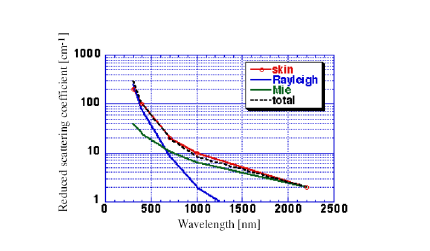
\includegraphics[width = 0.7\textwidth]{Chapter2/Figures/RayleighMieSkin.png}	
	\caption{Relation between reduced scattering coefficient, Mie scattering and Rayleigh scattering \cite{jacques1996origins}}
	\label{fig:RayMieSkin}
	\end{figure}
 Based on Fig.\ref{fig:RayMieSkin}, it is evidence that incident lights with longer wavelength could reach deeper in the skin. A complete survey on skin behaviour, properties and its appearance modelling is represented by \cite{igarashi2007appearance}. 
	
\section{Light Propagation Models in Skin}

Modelling the propagation of light in skin is a difficult and complex task, as a result several models have been proposed so far. 
Incident light in interaction with skin, is either reflected, refracted, scattered or absorbed. The two terms reflection and refraction are very close and simply can be confused. It should be considered that reflection occurs when waves bounce off a surface and travel onward with new angle and could be specular or diffuse. On the other hand refraction occurs when the light speed is changing as well as its direction. 
The reflected light from a surface is generally modelled by Dichromatic Reflection Model \cite{klinker1990physical}. This model describes total reflection as a combination of surface reflection (specular reflection, \% 5 for skin medium) and body reflection, which is reflected from the body of the medium (diffuse, \% 95 in the case of skin).  

	\begin{equation}
	 L_{Ref} = L_{Ref, Sur} + L_{Ref, Body}
	 \label{eq:LRef}
	\end{equation}

Considering different cases of light interaction with skin, and knowing the absorption and scattering coefficients of different skin layers and components, a propagation model can be modelled. Several models have been proposed including, the radiative transfer equation, monte carlo simulation, kubelka-monk model and modified bear lambert law. These models are discussed in the next section.  

\subsection{Radiative Transfer Equation Model}

The Radiative Transfer Equation (RTE) is referred to the mechanism of exchanging energy between atmosphere and underlying surface and between different layers of atmosphere. This model describes how the physical properties of the material are coupled to the measured spectrum. This model is commonly employed to model light propagation in scattering media. It is also used for modelling neutron propagation in nuclear reactor and propagation of gas in the atmosphere. 

In this model, the light is expressed in terms of its average energy after interacting with media and multiple scattering and it is defined in terms of intensity instead of electromagnetic field (see Eq.\ref{eq:LightAFSca})
	\begin{equation}
	dP = I(r,\hat{s},t)d\Omega da 
	\label{eq:LightAFSca}
	\end{equation}
In the above equation, $dP$ is the light power at time $t$ which is propagating along direction $r$ to meet the particle at section $da$. The section $da$ is considered in a cone with solid angel $d\Omega$, which is oriented along the unit vector $\hat{s}$. This vector is normal to the surface area of $da$. $I(r,\hat{s},t)$ is the light power (quantity of photon) per unit area per unit solid angle. Equation \ref{eq:LightAFSca} represents the light energy in terms of geometry, however this equation can be represented based on scattering ($\mu_{s}$) and absorption ($\mu_{a}$) coefficients of the media and phase function as well.

RTE model considers that only one type of particle is responsible for the scattering and absorption and the phase function is approximated by the Henyey Greenstein function. This model is considered as the most correct equation for representing the propagation of light in skin, however due to its complexity its direct impact had been rare in previous research. 
Radiative transfer equation is defined using transport equations such as Boltzmann equation. In this formulation, light propagation is considered as a photon flux which can be absorbed or scattered by the biological medium. 
	\begin{equation}
	s.\vec{\bigtriangledown}(r,\hat s ) = -(\mu_{a}+\mu_{s})I(r,\hat s)+ \frac{\mu_{a}+\mu_{s}}{4\pi}\int_{4\pi} p(\hat s,\hat s')I(r,\hat s )d\Omega'
	\label{Eq:Boltzmann}
	\end{equation}		
	
RTE due to its integral differentiation nature tends to be rather complex and often intractable without exact analytical solutions. Although efficient numerical method could be crucial, approximation analytical methods are available, such as transfer matrix method, singular eigenfunction method, perturbation method and etc.

Besides these methods several numerical techniques also have been used such as Monte Carlo method which is described in the next section. 

\subsection{Monte Carlo Method}
Monte Carlo (MC) methods are stochastic techniques. These methods take use of random variables and probability statistics to investigates the problems. These methods are useful to find numerical solutions to some problems which are analytically impossible or very complicated to solve. Monte Carlo method was first developed by Metropolis and Ulam \cite{metropolis1949monte} to simulate physical processes using a stochastic model. MC methods are used in different fields from economic, nuclear physics to regulating the flow of traffic. Monte Carlo is not represented by a specific technique and the term is applied to a wide range of techniques that can be applied. Although these techniques could be different , they all should follow the certain pattern:  

	\begin{itemize}
	\item A range of possible inputs are introduced to the system
	\item A set of random variables are produced by considering the introduced input ranges. 
	\item A series of mathematics calculations and statistics are performed using the random variables and inputs	
	\item The computed results of each calculation is integrated in the final answer
	\end{itemize}

%%Numerical methods that are known as Monte Carlo methods can be loosely described as statistical simulation methods, where statistical simulation is defined in quite general terms to be any method that utilizes sequences of random variables to perform the simulation.	Accordingly all the MC methods rely on a good random variables and by simulating more data, they gradually converge to a better estimation. 

Wang and Jacques et al. \cite{wang1992monte} introduced the earlier formulation of MC methods for multi-layered tissues. Figure \ref{fig:MC-Jacques} shows how they used their simulation to model the propagation of a photon through a homogeneous multi-layered medium (MCML).
	\begin{figure}[h]
	\centering 
	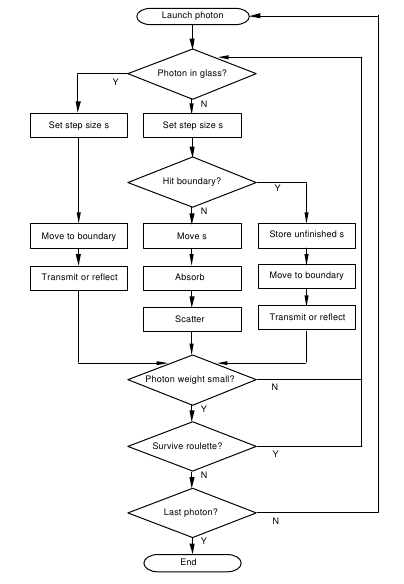
\includegraphics[width = 0.7\textwidth]{Chapter2/Figures/MCMLFelowChart.png}	
	\caption{Felow chart of MC method for multi-layered tissue \cite{wang1992monte}}
	\label{fig:MC-Jacques}
	\end{figure} 
	
Their approach later was used by \cite{tsumura2001mapping} for modelling the skin reflectance and mapping the skin pigmentation. The application of MC methods for modelling the light propagation through skin can be found in several articles \cite{meglinski2003computer, igarashi2007appearance}.

The MC simulations statistically computes the optical pathway of each photon, repeatedly with many iterations in order to find accurate results. Assuming that the photon is injected into a scattering medium, MC methods estimates the optical photon paths in an iterative manner based on parameters such as $\mu_{s}$ and $\mu_{a}$ and the phase function. This method can be computationally expensive, considering numerous iterations (often in the order of millions) are required for accurate results. Another disadvantage of the method is the noise introduced by the stochastic approach. Due to this matters, analytical methods might be more preferable, although they require more assumptions. 

%%We have simulated diffuse reflectance spectra of skin by assuming a
%%wavelength-independent scattering coefficient for the different skin tissues and
%%using the known wavelength dependence of the absorption coefficient of oxy-
%%and deoxyhaemoglobin and water. A stochastic Monte Carlo method is used
%%to convert the wavelength-dependent absorption coefficient and wavelength-
%%independent scattering coefficient into reflected intensity. The absorption
%%properties of skin tissues in the visible and near-infrared spectral regions
%%are estimated by taking into account the spatial distribution of blood vessels,
%%water and melanin content within distinct anatomical layers. The geometrical
%%peculiarities of skin histological structure, degree of blood oxygenation and the
%%haematocrit index are also taken into account. We demonstrate that when the
%%model is supplied with reasonable physical and structural parameters of skin,
%%the results of the simulation agree reasonably well with the results of in vivo
%%measurements of skin spectra.
%%
%%
%%The reflectance spectra of the human skin in visible and near-infrared (NIR) spectral region have been calculated
%%using the Monte Carlo technique, and the specular and internal reflection on the medium surface is taken into account.
%%Skin is represented as a complex inhomogeneous multi-layered highly scattering and absorbing medium. The model
%%takes into account variations in spatial distribution of blood, index of blood oxygen saturation, volume fraction of
%%water and chromophores content. The simulation of the skin tissues optical properties and skin reflectance spectra are
%%discussed. Comparison of the results of simulation and in vivo experimental results are given.

\subsection{Kubelka Munk Model}
The Kubelka-Munk (K-M) theory is one of the most popular and simplest approaches for computing the light transport in highly scattering medium. This theory was first developed by \cite{kubelka1931article}. In this article Kubelka and Munk introduced their theory based on the relationship between the scattering and absorption coefficients of layers of paint and its overall reflectance. K-M theory describes the radiation transfer in diffuse scattering media, by applying energy transport equations. K-M theory allows the quantitative studies of absorption, scattering and luminescence in diffuse scattering media and was used by different groups to skin analysis \cite{krishnaswamy2004biophysically,igarashi2007appearance,doi2003spectral,vyas2012computational,jolivot2011developpement}. 
K-M model has an analytical approach and is able to determine rapidly the skin optical parameters, using inversion approaches. 
The K-M model measures reflectance and transmittance of incident light in a scattering media, by relating the medium optical properties and K-M equations. This model considers three ways of interaction between incident light and the medium (reflection, absorption and transmission) and considers that the incident light flux is dividing into two fluxes ($I$, $J$), which are passing in two opposite direction in a medium (see Fig. \ref{fig:KMfig}). The energy variation of these fluxes over an infinitely small distance ($d$) are defined by the K-M equations:
	\begin{subequations}
	\small
	\begin{align}
	dI = (-kI-sI +sJ)dx\\
	-dJ = (-kJ -sJ+sI)dx
	\end{align}
	\label{Eq:KMEq}
	\end{subequations} 
	
	\begin{figure}[h]
	\centering 
	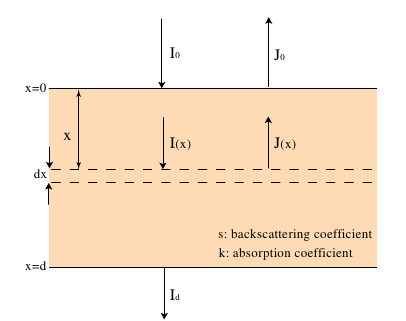
\includegraphics[width = 0.6\textwidth]{Chapter2/Figures/KMfig.png}	
	\caption{Illustration of light transport in an optical medium modele based on Kubelka–Munk theory. $I$ and $J$ illustrate diffuse fluxes travelling in the forward and backward directions,respectively. $s$ and $k$ are the backscattering and absorption coefficients of the medium,respectively and d is the sample thickness. \cite{igarashi2007appearance}}
	\label{fig:KMfig}
	\end{figure} 
	
Where $I$ is the light intensity inside the sample going downward (transmitted) and $J$ is the light intensity inside the sample going upward (backscattered). $s$ and $k$ are the scattering and absorption coefficients per unit thickness respectively and $x$ is the distance of the interaction. 

The reflectance ($\frac{J_{0}}{I_{0}}$) and transmittance ($\frac{I_{d}}{I_{0}}$) of the medium are related to the scattering and absorption coefficients as :

	
	\begin{subequations}
	\small
	\begin{align}
	R = \frac{(1-\beta ^{2})(exp(Kd)-exp(-Kd))}{(1+\beta) ^{2}exp(Kd)-(1-\beta) ^{2}exp(-Kd)}\\
	T = \frac{4\beta} {(1+\beta)^{2}exp(Kd)-(1-\beta)^{2} exp(-Kd))}\\  
	K = \sqrt{k(k+2s)} \hspace{0.7cm},\hspace{0.7cm}  \beta = \sqrt{\frac{k}{k+2s}}
	\end{align}
	\label{eq:RTKB}
	\end{subequations}


Kubelka-Munk theory assumes that the sample possesses inhomogeneities, which are small compared to its thickness and incident radiation is diffused and the regular reflection at the boundaries can be neglected \cite{jolivot2011developpement}. Due to these assumptions, it causes false estimations in certain cases, for instance this model overestimates the radiance of scattered light in a medium with high albedo (strongly anisotropic scattering medium), such as superficial area of the skin \cite{igarashi2007appearance}. This method can not predict the spatial distribution of light due to scattering as well, since only two scattering direction of light is considered. 
However due to its simplicity, speed and its extension to NIR \cite{cotton1997noninvasive}, it has been used by different groups for modelling the light transport through the skin and retrieving internal parameters such as epidermal melanin, dermal blood, papillary dermal thickness \cite{cotton1997noninvasive,jolivot2011developpement}



%%%The scattering and absorption coefficient can be written in terms of reflection and transmittance parameters as it is stated by Eq. \ref{Eq:SK-RT}
%%%	
%%%	\begin{subequations}
%%%	\small
%%%%	\begin{center}
%%%	\begin{align}
%%%	\frac{S}{K} = \frac{1+R^{2}-T^{2}}{2R}-1\\
%%%	S.t, \hspace{0.1cm} layer_{thickness} \gg 0, \hspace{0.1cm} T = 0	,  \hspace{1cm} \frac{S}{K} = \frac{(R-1)^{2}}{2R} 
%%%	\end{align}
%%%%	\end{center}
%%%	\label{Eq:SK-RT}
%%%	\end{subequations} 
%%%
%%%
%%%The equations \ref{Eq:SK-RT} can be extended for two and more $n$ layers. The total remittance $R_{1,2}$ and transmittance $T_{1,2}$ for two layers which is based on the reflectance and transmittance of each layer is stated in the following equation: 
%%% 	
%%%	\begin{subequations}
%%%	\small
%%%	%\begin{center}
%%%	\begin{align}
%%%	R_{1,2} =R_{1} + T_{1}T_{2}R_{2}(1+R_{1}R_{2} + R_{1}^{2}R_{2}^{2}+\ldots) = R_{1} + \frac{T_{1}^{2}R_{2}}{1-R{1}R_{2}}\\
%%%	T_{1,2} = T_{1}T_{2}(1+ R_{1}R_{2} + R_{1}^{2}R_{2}^{2}+\ldots) = \frac{T_{1}T_{2}}{1-R_{1}R_{2}}
%%%	\end{align}
%%%	%\end{center}
%%%	\label{Eq:TR2}
%%%	\end{subequations} 
%%%
%%%Equation \ref{Eq:TR2} can be extended for n layers such as: 
%%%	\begin{subequations}
%%%	\small
%%%	%\begin{center}
%%%	\begin{align}
%%%	R_{1,2,\ldots n} =R_{1,2,\ldots n-1} + \frac{T_{1,2,\ldots ,n-1}^{2}R_{n}}{1-R_{1,2,\ldots, n-1}R_{n}}\\
%%%	T_{1,2,\ldots n} = \frac{T_{1,2,\ldots n-1}T_{n}}{1-R_{1,2,\ldots, n-1}R_{n}}
%%%	\end{align}
%%%	%\end{center}
%%%	\label{Eq:TRn}
%%%	\end{subequations} 

\subsection{Modified Beer-Lambert Law model}

Beer-Lambert law is modelling the light transport in an optical medium, assuming the scattering is small and absorption effects is much greater than scattering. In this case the incident light goes directly into the medium and gets attenuated exponentially due to absorption \cite{igarashi2007appearance}. This law is written as: 
	\begin{equation}
	 L = (1-R_{F})E exp(-\mu_{t}d)
	\label{eq:BL}
	\end{equation}
where $L$ is the radiance, $E$ is incident radiance, $R_{F}$ is the coefficient of Fresnel reflectance for normal light incidence and d is the thickness of the optical medium. This model works well when absorption coefficient is at least 10 times greater than scattering coefficient which is the condition when skin is illuminated in ultraviolet and far infra-red light and does not hold for the visible and near infra-red illumination. Since this model is invalid for modelling the light transport in skin, the modified Beer-Lambert law was proposed \cite{igarashi2007appearance}.

The modified Beer-Lambert law is considering highly scattering medium and since the optical path length in a highly scattering medium is not the same as the medium thickness it modified the original formula by considering the mean path length of the scattered light $d(\lambda)$, 
	\begin{equation}
	 L = (1-R_{F})E(\lambda) exp(-\mu_{a}d(\lambda))
	\label{eq:BL}
	\end{equation}

The modified Beer-Lambert law was used by \cite{meglinski2003computer,shimada2001melanin,tsumura2003image} in order to model the light transport in skin. In \cite{meglinski2003computer} it was shown how modified Beer-Lambert law uses linear equation to relate the tissue attenuation with its absorption coefficient. In this relation, $\rho$ is the space between the source and the detector and $\sigma$ is the scaling factor, $G$ is an offset term determining either the tissue probe geometry or the scattering coefficient. This equation can be extended for N chromophores as well (see Eq.\ref{Eq-BLA}.b) and the properties of theses chromophores can be obtained by measuring $A$ with a minimum N+3 wavelengths and using multi-linear regression. In this equation, $\mu_{a}$ is represented as sum of absorption coefficient for each choromophore, which is determined by the concentration ($C_{i}$) and specific absorption coefficient ($\epsilon_{i}$) of each choromophore.  

	\begin{subequations}
	\begin{align}
	 A = -ln \frac{I}{I_{0}} = \mu_{a} \sigma_{\rho} + G\\
	 A = a + b\lambda + \sum_{i=1}^{N} C_{i}\epsilon_{i}(\lambda)
	 \end{align}
	\label{Eq-BLA}
	\end{subequations}

%%% Local Variables: 
%%% mode: latex
%%% TeX-master: "../thesis"
%%% End: 